\documentclass{article}\usepackage[]{graphicx}\usepackage[]{color}
%% maxwidth is the original width if it is less than linewidth
%% otherwise use linewidth (to make sure the graphics do not exceed the margin)
\makeatletter
\def\maxwidth{ %
  \ifdim\Gin@nat@width>\linewidth
    \linewidth
  \else
    \Gin@nat@width
  \fi
}
\makeatother

\definecolor{fgcolor}{rgb}{0.345, 0.345, 0.345}
\newcommand{\hlnum}[1]{\textcolor[rgb]{0.686,0.059,0.569}{#1}}%
\newcommand{\hlstr}[1]{\textcolor[rgb]{0.192,0.494,0.8}{#1}}%
\newcommand{\hlcom}[1]{\textcolor[rgb]{0.678,0.584,0.686}{\textit{#1}}}%
\newcommand{\hlopt}[1]{\textcolor[rgb]{0,0,0}{#1}}%
\newcommand{\hlstd}[1]{\textcolor[rgb]{0.345,0.345,0.345}{#1}}%
\newcommand{\hlkwa}[1]{\textcolor[rgb]{0.161,0.373,0.58}{\textbf{#1}}}%
\newcommand{\hlkwb}[1]{\textcolor[rgb]{0.69,0.353,0.396}{#1}}%
\newcommand{\hlkwc}[1]{\textcolor[rgb]{0.333,0.667,0.333}{#1}}%
\newcommand{\hlkwd}[1]{\textcolor[rgb]{0.737,0.353,0.396}{\textbf{#1}}}%
\let\hlipl\hlkwb

\usepackage{framed}
\makeatletter
\newenvironment{kframe}{%
 \def\at@end@of@kframe{}%
 \ifinner\ifhmode%
  \def\at@end@of@kframe{\end{minipage}}%
  \begin{minipage}{\columnwidth}%
 \fi\fi%
 \def\FrameCommand##1{\hskip\@totalleftmargin \hskip-\fboxsep
 \colorbox{shadecolor}{##1}\hskip-\fboxsep
     % There is no \\@totalrightmargin, so:
     \hskip-\linewidth \hskip-\@totalleftmargin \hskip\columnwidth}%
 \MakeFramed {\advance\hsize-\width
   \@totalleftmargin\z@ \linewidth\hsize
   \@setminipage}}%
 {\par\unskip\endMakeFramed%
 \at@end@of@kframe}
\makeatother

\definecolor{shadecolor}{rgb}{.97, .97, .97}
\definecolor{messagecolor}{rgb}{0, 0, 0}
\definecolor{warningcolor}{rgb}{1, 0, 1}
\definecolor{errorcolor}{rgb}{1, 0, 0}
\newenvironment{knitrout}{}{} % an empty environment to be redefined in TeX

\usepackage{alltt}
\usepackage{Sweave}
\usepackage{float}
\usepackage{graphicx}
\usepackage{tabularx}
\usepackage{siunitx}
\usepackage{mdframed}
\usepackage{natbib}
\bibliographystyle{..//refs/styles/besjournals.bst}
\usepackage[small]{caption}
\setkeys{Gin}{width=0.8\textwidth}
\setlength{\captionmargin}{30pt}
\setlength{\abovecaptionskip}{0pt}
\setlength{\belowcaptionskip}{10pt}
\topmargin -1.5cm        
\oddsidemargin -0.04cm   
\evensidemargin -0.04cm
\textwidth 16.59cm
\textheight 21.94cm 
%\pagestyle{empty} %comment if want page numbers
\parskip 0pt
\renewcommand{\baselinestretch}{2}
\parindent 15pt

\newmdenv[
  topline=true,
  bottomline=true,
  skipabove=\topsep,
  skipbelow=\topsep
]{siderules}
\IfFileExists{upquote.sty}{\usepackage{upquote}}{}
\begin{document}
\title{Life History Theory and Floral-Foliate Phenological Patterns in Temperate Forest Trees}
\author{Daniel Buonaiuto}
Daniel Buonaiuto
\par OEB 53
\par\data{\today}

Green is the color of spring, but any keen observer walking the temperate, deciduous forest of the Eastern United States early in the season would readily witness that it is often the subtle whites, reds and yellows of emerging tree flowers that are the first harbingers of spring in temperate forest communities. In some deciduous tree species, seasonal flowering proceeds leaf development, while in others, it is leaf expansion that occurs first. The study of phenology, the timing of annual life cycle events, has a long history, and even in the late 1800's, naturalists speculated that such contrasting floral-foliate sequences were not merely incidental, but that these patterns, in and of themselves, may be adaptive \citep{Robertson1885}. However, despite increasing scientific interest in the study of phenology over the past several decades, the phenology of reproductive (flowering, fruiting) and productive (bud burst, leaf out and drop) stages have long been treated separately, and both the mechanisms and effects of floral-foliate phenological patterns remain poorly studied empirically \citep{Wolkovich2014}.
\par Even finding suitable language to describe floral-foliate patterns in the existing literature is an difficult endeavor. Early botanical dictionaries define flowering followed by leaves as both "proterany" and "hysteranthy" (which grammatically should be antonyms). Other describe flowering before leafing as "precocious" flower, but that term can also refer to flowering early in ontogeny and have nothing do do with seasonality. To the aim of maintaining a consistency of usage, I will adopt the terminology used by Lamont and Downes \citeyear{Lamont2011} in which proteranthy refers to flowering before leafing, synanthy refers to flowering and leafing simultaneously and seranthy refers to flowering after leafing.
\par As global climate is predicted to change dramatically in the comping decades It is imperative that we, as scientists, better understand these phenological patterns.The effects of climate change have already appeared in phenology \citep{Menzel2006} and the degree to which these phenological shifts are altering floral foliate sequences is virtually unknown. If the sequences themselves are indeed adaptive, conferring a significant fitness benefit to individuals under historical conditions, disruptions to these patterns cause by changing climate conditions could have negative demographic consequences for many forest tree species. To better understand the importance of these sequences and the ability for species to maintain them in a changing world, researchers should focus their attention on gaining a more complete picture of mechanisms and effects of this. To this end, in section one of this paper, I will first present the dominant hypothesis for proteranthy in the context of life history theory, and them evaluate the empirical and theoretical evidence for its support. In section two, I will discuss some of the biological mechanisms producing the phenological patterns we see today and discuss how they may enable or constrain plastic responses to changing climate in forest trees.
\section{Proteranthy and Life History Theory}
\par Life history theory seeks to explain how organisms achieve reproductive success. The classical theory is based on an optimization model- life history traits of organisms (for example: age of reproduction, seed size) are determined by trade offs in both extrinsic (environmental, community) and intrinsic (genetics, physiology) factors, which result in a lineage specific optimum for life history characters \citep{Stearns2000}.  Typically, life history theory is applied to the full lifespan of an organism, and in the context of plants, has been applied concerning the transition between vegetative growth and reproductive life stages for annual plants \citep{Glover2014}. But trees, being long lived, perennial organisms, do not experiences the abrupt transitions, and the interplay between vegetative and reproductive development is far more "fuzzy". That said, I will attempt to apply this model of discrete reproductive optimization the context of seasonal context, appropriate for tree phenology.
 Before I go on, we should consider the environmental conditions that typically induce phenological responses. For temperate woody plants, it is generally accepted that the dominant cues for spring phenological events such as flowering and leaf out are vernalization temperatures (in winter), forcing temperatures (in spring) and photoperiod, but it is clear that the interactions between these cues are complex, and behave differently for different species and in different locations \citep{Forrest2010}. Optimization of phenological timing depends on how trees accurately "interpret" these cues as reliable signals of overall seasonal patterns. For example, warm temperatures are only reliable cues if they tend to coincide the with onset of spring. As such, periodic warm spells in the heart of winter could "fool" plants into initiating phenological events in a sub-optimal season. It is therefore assumed that trees have locally adapted different sensitivities to these cues combinations, and selection maintains individuals that interpret their environment successfully. 
\par For flowering alone, optimization in a seasonal environment depends on several evolutionary drivers. For flower tissues and ultimately reproductive output, there is likely tradeoff between flowering minimizing risk for early season frost damage and maintaining enough time for fruit development and dispersal. The timing is further selection by the vectors of pollination and interactions with antagonists \citep{Austen2017}.  Considering leaf phenology alone, optimization is though to maximize the growing season and minimizing the risk of damage from late season frost \citep{Kramer1995}. 
But now we must consider the timing of leaves and flowers together. Might the presence of leaves change the behaviors of pollen vectors? Might the presences of flowers with out leaves change the resource allocation dynamics? The sequencing of leaves and flowers, in and of itself, produces its own set of tradeoffs, which I will now discuss as we review the main hypothesis about proteranthy.
\par Proteranthy is thought to be an adaptation for pollination efficiency. Theorists explain that this trait is common in wind pollinated species, because producing flowers in the leafless state allows for maximum wind flow through the canopy and significantly reduces the potential for pollen interception by non-floral parts \citep{Rathcke1985, Whitehead1969}.Though proteranthy is often discussed in the context of wind pollination, similar theory could be applied to insect pollinated species in that tree flowers are easier for pollinators to located when there are no leaves as barriers or obstacles. Presumably, more efficient pollination would allow for species to reduce their overall investment in reproduction. However, their would still be costs associated with this life history trait. Proteranthous flowering would only be effective if it occurred before the community as a whole leafed out, which would push such flowering early into the season to a time when risk of frost damage is high. Additionally, proteranthous flowering probably has an energetic cost, taking place at a time of the year when stored carbohydrates are at their lowest, with out the assistance of supplemental carbon from foliar photosynthesis\citep{Aschan2003}.
To my knowledge, there have been no empirical studies testing the fitness benefits of proteranthy, but several studies seem to support it though indirect evidence. There is evidence that wind pollination, a derived trait in angiosperms, arose at the same time as decidiousness \citep{Whitehead1969}. While this fact doesn't address proteranthy directly, it can be argued that this coincidence indicates that a leafless season is a necessary condition for wind pollination. This evolutionary argument can be supplemented by a observation from biogeography that wind pollination is rarely found in the tropics, and common in the temperate and boreal zones where there is a leafless season \citep{Whitehead1969}.
\par Other studies have more directly measure changes in pollen interception by non-floral plants structures at different stages of canopy closure. \citep {Tauber1967, Milleron2012}, and found strong evidence for filtration of pollen by no reproductive structures canopy closure increased. These studies provide evidence that canopy fill does create a significant barrier to pollen transfer in forest, but fall short of concretely supporting the adaptive significance of proteranthy because they are not able to quantify the direct effects of pollen filtration on tree fitness.
\par Another approach to obtain indirect evidence of a fitness benefit of proteranthy is to use a comparative morphology approach between closely related proteranthous and seranthous species. The approach was applied in the insect-pollinated dogwoods (Genus: \textit{Cornus}) which show a diversity of floral-leaf sequences within the genus \citep{Gunatilleke1984}. While the only three species were compared, the authors found evidence for a tradeoff between pollination efficiency and floral investment with proteranthous flowering \textit{Cornus mas} showing a reduced floral diameter and peduncle length when compared to synthanous \textit{Cornus florida} and seranthous \textit{Cornus sericea}. There are now techniques to quantify investment in tissues and trace structural carbon movement throughout plant organs, and with such tools, these kind of comparative studies applied more broadly in clades with diverging floral-foliate sequences, would aid our understanding of proteranthy tremendously.
\section{Floral and foliate phenologies: independent or constrained?}
\par We understand that phenological stages (hence: phenophases) are not optimized in a vacuum, but timing is depends on both leaf and flower physiology and the functional relationship between them. Climate change is already having dramatic impact on phenology \citep{Wolkovich2012} Will flowering and leafing phenophase shift relative to each other, maintaining their optimized temporal relationship or will new patterns emerge?
At the heart if this inquiry is the question: to what degree is the timing of one phenophase constrained by the other? A broad observation of temperate forest trees shows significant degree of correlation. Generally, years of earlier leafing than average also are years with earlier flowering than average \citep{Lechowicz1995}, but because of high seasonal variability and complex ecological interactions observational studies cannot assess whether these patterns are incidental, a product of independent timing of flowering and leafing, or determinate, a product of biological constraints between phenophases. 
\par As I mentioned above, both floral and foliate phenophases respond to same environmental cues. This fact alone could explain the phenotypic correlation between flowering and leaf out timing, through or a overlapping regulatory mechanism, perhaps though pleiotropy or some shared genetic pathway for phenology that influences both flowering and leaf out timing. Considering the later first-- it is important to point out that due to their long generations times, trees have not been historically amenable to genetic research. Most of our knowledge about the genetics responsible for phenological responses to the environment come from studies in model organism \textit{Arabidopsis thaliana}. One study of particular relevance, sought to understand how climate conditions (vernalization) might similarly effect the timing of two discrete life history stages,germination and flowering time\citep{Auge2017}. The authors found that genes in the flowering pathway did indeed pleiotropically regulate seed germination. However, few assays found a consistent response to vernalization between the two stages, and in many cases, the response to vernalization was reversed across life stages. As such, the authors conclude that the vernalization genes regulate the different life stages of \textit{Arabidopsis} with a degree of independence. 
\par To my knowledge the only genomic based study of phenology in trees was performed in the proteranthous model species \textit{Populus trichocarpa}. These studies identified one gene FT1 which induced a flowering response due to vernalization, and an FT2 gene, which facilitates the vegetative growth and autumn dormancy induction as a response to photoperiod \citep{Glover2014}. While this result is promising because apparent homologs in \textit{Arabidopsis}, it has been suggested that the pathways that regulate the flowering response to environmental signals are poorly conserved with extreme  difference among species within species \citep{Blackman2017}, and as such, it is not possible to suggest any generalities based on the current body of research in this area.
\par I have previously stated that one possible explanation for the floral-foliate patterns we see today is that they are incidental, produced by independent responses to environmental cues. Within the reaction norms of the current climate space, these patterns may appear to be relatively fixed, but if floral and foliate phenophases are differentially sensitive the environmental cues, and seasonal temperatures change significantly as they are expected to do in the coming decades, the patterns may be disturbed. There is one case study that would reassure us; a study in two cherry family species (genus \textit{Prunus}) found that the different timing of floral and vegetative bud break could be explained by differential sensitivities to spring warming \citep{Guo2014}. If this is the case, we would expect to see these patterns maintained even in an era of global climate change.
\par However, as I mentioned above, there is tremendous variation in how species, and populations within species, respond to climate cues, so I set out to further test the independence of phenological responses between floral and foliate phenophases. I performed a small pilot in which growth chambers were used to subject three species of woody, deciduous shrubs to four different temperature and photoperiod treatment combinations and compared the phenological response of flower and leaves. Floral and foliate phenological responses were differentially affected by changing combinations environmental cues, and  the degree of divergence of these responses varied significantly among species. One species, mountain holly  (\textit{Ilex mucronata}), seemed to maintain the temporal offset between leafing and flowering relatively consistently under different treatment combinations. At the other extreme, floral phenology  of beaked hazelnut (\text{Corylus cornuta}) was most sensitive to photoperiod, while foliate phenology was more sensitive to forcing temperature, which under some conditions resulted in a complete reversal to the floral-foliate sequence (result pictured in the figure below)
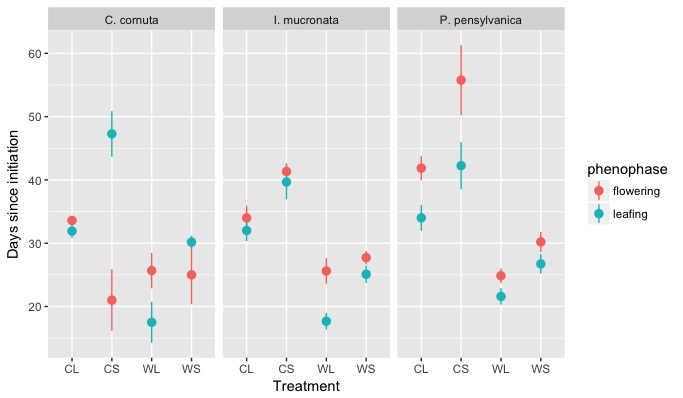
\includegraphics[width=16cm,height=7cm] {shrubs_4_csee}
These results suggest that floral and foliate phenophases can respond to the environment relatively independently of each other, each one tracking its own climate optimum, but that the degree of independence varies significantly among species. 
\par It is important to pause and reflect that we cannot yet judge the adaptive significance of having independent or constrained floral and foliate phenophases in an era of climate change. We can explore hypothetical scenarios to illustrate this uncertainty. Consider proteranthous species with independent floral and foliate phenophases. This independence may allow each phenophase to be expressed at its own climatic optimum, but if, as in the case of beaked hazelnut, leafing is advanced by warming and flowering controlled by photoperiod, the overall impact will be a reduction duration of the leafless flowering period. If this state is, as we have explore above, critical for successful pollination in wind pollinated species, the overall impact of climate change in such taxa would be decreased reproductive success, which would ultimately have negative demographic consequences. But there may also be downsides to constrained phenophase expression. If phenology is tracking a warmer climate, proteranthous flowering would be pushed increasingly earlier, into a less stable climate space where frost events are more common. If tree flowering were to more often coincide with frost events, this too could reduce the overall fitness of an individual. Yet still, species who do not phenologically track climate change at all, will not benefit from an extended growing season, which could put them at a competitive disadvantage to species that do track. We cannot yet predict the likelihood of these scenarios, and just like all other aspects of community dynamics, the boundaries are likely to be fuzzy. However it is clear, that alterations to phenological patterns may significantly impact community dynamics in an era of global climate change.



\bibliography{..//refs/oeb53}
\end{document}
